\chapter{Anthropodidactic learning: Auto-ALS}
\label{ch:auto-als}
\todo{Make sure a research question is explicitly mentioned}
\todo{Make sure Aki's comments are copied as TODOs}
\todo{Ensure standard nomenclature}

\section{Anthropodidactic learning: a modest proposal}


\subsection{What is anthropodidactic learning?}

\emph{Anthropodidactic machine learning} is using didactic materials
developed for human students (textbooks, lectures and/or lecture notes,
explanations, homeworks, exercises, \href{http://www.virtu-als.com/}{games} and other
sorts of interactive edutainment) to train artificial intelligence.
Examples of anthropodidactic learning include using language textbooks
to train a machine translation model or using a flight simulator
developed for pilot training to train an autopilot with reinforcement
learning \href{https://openreview.net/pdf?id=H1mMHwt9X}{{[}Staudinger
Jorgensen Margineantu 2018{]}}.


\subsection{Why should anyone care?}\label{why-should-anyone-care}

Because the education industry puts a lot of effort into curating and
systematising knowledge in a way that can be useful for any learner,
whether they run on
\href{https://en.wikipedia.org/wiki/Human_brain}{carbon-} or
\href{https://en.wikipedia.org/wiki/Central_processing_unit}{silicon-based}
hardware. For example: - Exercise sets in mathematics, physics and
language learning, to name a few fields, are explicitly designed to
cover all important clusters/corner cases of the subject area -
something that isn't guaranteed in most datasets like logs, business
records or text corpora. - Exercise sets are also sorted by difficulty.
This creates a useful curriculum
\href{https://arxiv.org/abs/2101.10382}{{[}Soviany 2021{]}} to follow
when training a machine learning model. - Educational software aims to
give users immediate and precise feedback on their mistakes: delayed
gratification, as it turns out, is hard for
\href{https://en.wikipedia.org/wiki/Stanford_marshmallow_experiment}{people}
and reinforcement learning algorithms
\href{https://www.nowpublishers.com/article/Details/PGL-010}{{[}Gulwani
et al 2017{]}} alike.

See The Art of Problem Posing
\href{https://www.taylorfrancis.com/books/mono/10.4324/9781410611833/art-problem-posing-stephen-brown-marion-walter}{{[}Brown,
Walter 2004{]}} to learn more about\ldots{} the art of problem posing.


\subsection{This has been done already, hasn't it?}\label{this-has-been-done-already-hasnt-it}

Machine learning community is undoubtedly interested in taking lessons
from human learning, efforts to do so bear the umbrella term of
\href{https://ieeexplore.ieee.org/document/8481253}{antropomorphic
machine learning}. The prime example is curiculum learning
\href{https://arxiv.org/abs/2101.10382}{{[}Soviany 2021{]}}: it was born
with the observation that the order in which data is presented to human
students is crucial for them achieving their learning goals, so perhaps
it makes a difference for machines too.

However, examples of directly reusing learning aids developed for human
students are hard to come by. A notable exception is Reinforcement
Learning where decision-making agents are often trained on games
initially intended for people. And while the claim that
\href{https://gym.openai.com/envs/\#atari}{Atari games} and
\href{https://www.microsoft.com/en-us/research/project/project-malmo/}{Minecraft}
are educational material may be somewhat stretching the definition of
education, interactive simulators first developed for people and later
adapted for reinforcement learning include
\href{https://openreview.net/pdf?id=H1mMHwt9X}{X-plane} (used for
training pilots) and Virtu-ALS
\href{https://pubmed.ncbi.nlm.nih.gov/34977561/}{{[}Liventsev et al
2021{]}} (used for training nurses). Some antropodidactic work has also
been done in natural language processing, training language models on
children's books \href{https://arxiv.org/pdf/1511.02301.pdf}{{[}Hill et
al 2016{]}} and exercises for language learning
\href{https://aclanthology.org/2020.ngt-1.28.pdf}{{[}Mayhew et al
2020{]}} from \href{https://www.duolingo.com/}{Duolingo}

These examples, however, are exceptions rather than the rule and, in
general, anthropodidactic programming remains criminally underexplored.
A couple of research directions that seem extremely promising to me are:
- Training a language model on exercisebooks in subjects like
mathematics and the sciences to achieve a system capable of problem
solving in these fields. - Using beginner-level programming tasks to
develop program synthesis.

Didactic materials are a large class of useful data waiting for someone
to turn them into a successful artificial intelligence system/product.
Will it be \emph{you}, \%username\%?




\newpage
\section{Patient Simulators as Benchmarks}
\citeself{section}{liventsevEffectivePatientSimulators2021}

Benchmarks orient AI \cite{liangHolisticEvaluationLanguage2022}. Whether it's ImageNet \cite{dengImagenetLargescaleHierarchical2009} in Computer Vision or GLUE \cite{wangGLUEMultitaskBenchmark2018} in natural language processing, benchmarks are a core research tool in mature applications of machine learning, enabling quantitative analysis of learning methodologies to guide and orient their development.
Machine learning in Healthcare, an emergent field with unique challenges in availability of research datasets \cite{Anshik2021Handling, Gilbert2015market, Pahwa2021Big, Yazhini2019State} lacks an accepted benchmarking standard: recent literature reviews \cite{palMachineLearningHealthcare2023,tortorellaHealthcareTrendsChallenges2020} of the field cover a variety of studies that each use their own (often non-public) benchmark. The shortage of standard benchmarks has been consistently identified as a central roadblock for machine learning in Healthcare
\cite{Crown2015Potential, David2020Evaluating, guSupervisedLearningPervasive2023, harutyunyanMultitaskLearningBenchmarking2019, Kathrin2022Benchmark, liventsevEffectivePatientSimulators2021, mcdermottReproducibilityMachineLearning2021, purushothamBenchmarkingDeepLearning2018, S2017Benchmark}.

\newpage
\section{Auto-ALS}
\label{sec:virtu-als}

\citeself{section}{liventsevEffectivePatientSimulators2021}

\todo{Get technical details from github}

\begin{figure}
    \centering
    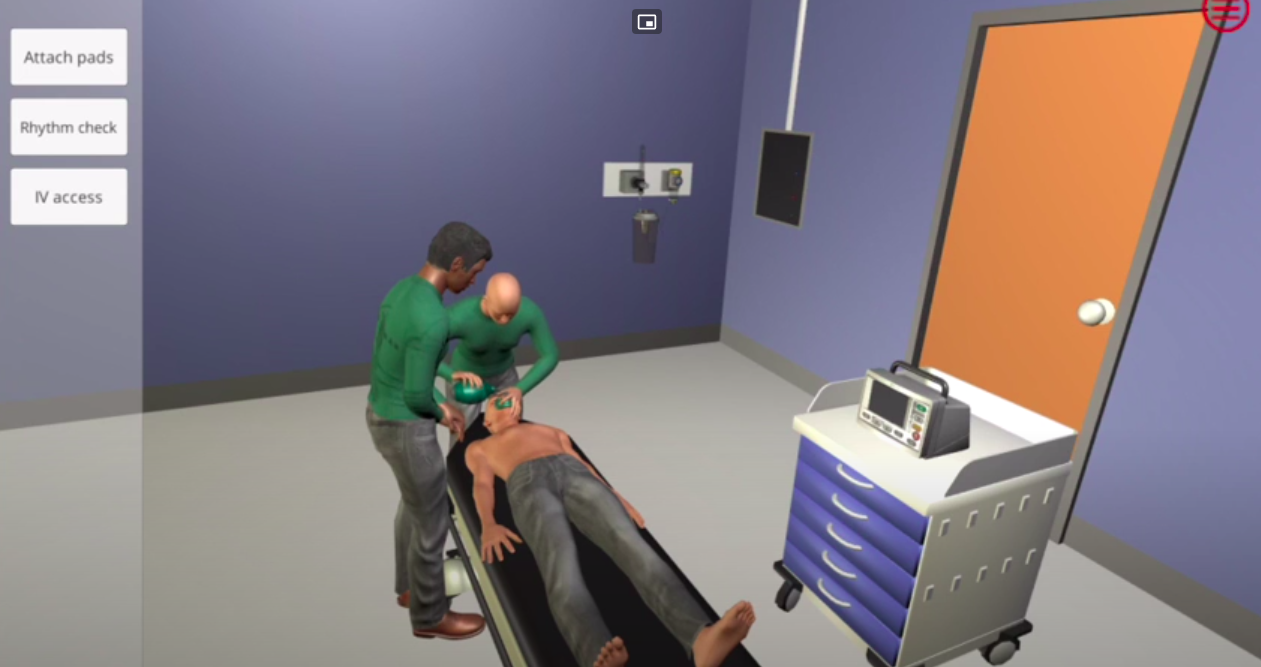
\includegraphics[width=\linewidth]{Virtu-ALS.png}
    \caption{Virtu-ALS}
    \label{fig:virtu-als}
\end{figure}

Virtu-ALS is a \emph{didactic} emergency care simulator mainly targeted at students and junior healthcare professionals, although its application as a reinforcement learning \emph{benchmark} was anticipated and accounted for by the authors \cite{briskAIEnhanceInteractive2018}.
Its most prominent feature is its visual nature (figure \ref{fig:virtu-als}): the user has access to a 3D-rendered virtual copy of a hospital room, view the monitor, press buttons on a defibrillator, etc.
However, the visual modality means that its observation space 
\begin{equation}
    \mathcal{O} \subset R^{307200}
\end{equation}

Such a high dimensionality of the observation space makes it an extremely challenging reinforcement learning task.
Tasks from this family have been solved with deep neural networks \cite{mnihPlayingAtariDeep2013}, however not only does it require a long and expensive training process, it also means that resulting treatment strategies are black box neural networks that no clinical expert understands.
This approach to decision making is extremely hard to introduce into clinical practice \cite{priceBigDataBlackbox2018,watsonClinicalApplicationsMachine2019}

Like most \emph{didactic} simulators, Virtu-ALS exhibits considerable \emph{confirmation bias} - any decision that's not supported by the standard emergency care protocol \cite{thimInitialAssessmentTreatment2012} is considered a mistake and rewarded negatively.

As our first model, we propose a low-dimensional version of \emph{Virtu-ALS}.
\emph{Auto-ALS} is a modification of Virtu-ALS that removes all the complexity of dealing with a visual 3D environment while retaining all the complexity of dealing with a patient that requires emergency care.
This is achieved by attaching an event listener to Virtu-ALS that registers all observable events that can occur in the simulator in response to the user's actions.
The events are listed in table \ref{tab:auto-als}, organized by which agent action can trigger which event.
\emph{Tick} is a special event that occurs every time the simulator is advanced a timestep, and is negatively reinforced, which when used with reinforcement learning algorithms discourages clinicaly unnecessary actions.

\begin{equation}
     o^{+} = \langle \rlobs_1 \in \rlobs_1, \exp(t_1-t), \dots, \rlobs_n \in \rlobs_n, \exp(t_n-t), \rangle
\end{equation}

where $\rlobs_i$ is the value of the observation and $t$ is current time and $t_i$ is time when observation $i$ (for $i=5$, \verb|ResponseGroan|) has \emph{last} occurred and $\exp(t_i-t)$ represents its decaying relevance.
For \emph{measurements}, the $\rlobs_i$ equals the magnitude of the measurement, however, for binary obsevations $\rlobs_i$ would always be equal to one.
For memory efficiency, for all $i$ that correspond to binary observations, $\rlobs_i$ is skipped from the $o^{+} $ vector and the actual observation vector $o$ has size $36+7*2=50$, as opposed to $36+7)*2=86$

\newpage
\subsection{Decision process}
\label{sec:mpdp}

Implementing Auto-ALS requires grappling with some of the limitations of POMDP framework (as described in section \ref{sec:ps-task-taxonomy})
\begin{enumerate}
    \item Some decision making scenarios legitimately have a discrete flow of time: a CPU, for example, makes a decision every $\frac{1}{\text{clock frequency, Hz}}$ of a second. However, most real-life decision making settings (such as the hospital setting) happen in a continuous time flow with no limits on how often or how rare actions and observations occur.
    \item The agent cannot respond to an observation with less than one (i.e.~zero) or more than one action. This can be fixed by modeling $\rlaction_n)$ as a set of actions.
\end{enumerate}

Both of these problems have been successfully addresed with artificial time discretization and complex action spaces $\rlactions$, however this is done on a case by case basis for each particular environment. A general model that addresses these challenges would be very useful.

\paragraph{Message Passing Decision Process}

Let us attach a timestamp $t$ to every observation, reward and action in the decision process, making them 2-tuples. An action $\langle a, t\rangle$ is a message from the agent to the environment, an observation $\langle \rlobs, t \rangle$ or a reward $\langle r, t \rangle$ is a message from the environment
to the agent. Messages can be sent as often or as rare as needed:

\begin{figure}
\centering
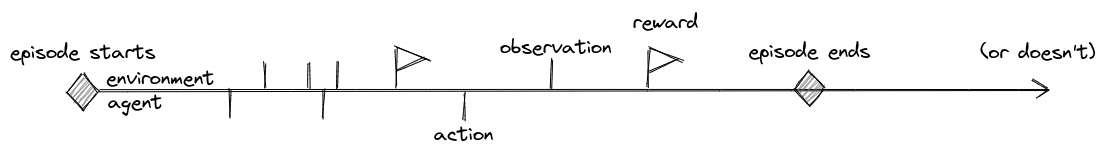
\includegraphics[width=\linewidth]{images/mpdp.png}
\caption{Message Passing Decision Process}
\end{figure}

Observations and actions are sampled from the \emph{environment} and
conditioned on the timestamp and all actions of the agent before that
time:

\begin{equation}
    \rlobs_t \sim p(\rlobs_t|t,\{\rlaction, t_\rlaction | t_\rlaction < t\})
\end{equation}

The actions are sampled from the \emph{agent}, also conditioned on the
timestamp and all observations before that time:

\begin{equation}
a_t \sim \pi(a_t|t, \{ o, t_o | t_o < t \})
\end{equation}

where $\rlobs_t \in O\^{}\{+\}$
and $a_t \in A\^{}\{+\}$

\begin{equation}
    O\^{}\{+\} = \{\text{no observation} \} \cup O 
\end{equation}

\begin{equation} 
A\^{}\{+\} = \{\text{noaction} \} \cup A 
\end{equation}

\paragraph{Discretization}

Now that we're done with the theory, it is a good time to remember that
we live in the real world and, in the real world, unless you plan to run
reinforcement learning algorithms on a
\href{https://royalsocietypublishing.org/doi/10.1098/rstb.2018.0372}{liquid
computer} (in which case, please let us know how it goes!), evaluation
of $\pi(a_t)$ will be done
either by a regular computer that can only evaluate it a finite number
of times a second or something even slower than that. Hence,
discretization is still desirable. However, we need a discretization
strategy that will make the resulting discrete decision process
equivalent (or at least as equivalent as possible) to the continuous
MPDP.

\paragraph{Decision schedules}

So we've established that the practicalities of implementing a
reinforcement learning algorithm mean that in any timeframe
$\langle t, t + \Delta t \rangle$ a finite number of decisions should
be taken. This can be achieved by a decision schedule that is some
combination of:

\begin{itemize}
\item
  making a decision every time any message from the environment
  (observation or reward) is received
\item
  making a decision at regular intervals
  $\Delta t$
\item
  after making a decision, scheduling a decision time
  $t_d$ later in the future
\end{itemize}

At every decision point the agent has to receive information about the
observations that recently occured and output some number of actions
(may be zero)

\paragraph{Observation space}

When an observation is modeled as $\langle \rlobs, t \rangle$, the most faithful way to represent the history of observations to the agent is

\begin{equation} 
\overrightarrow{\rlobs} = \langle \rlobs_1, t_1, \rlobs_2, t_2, \dots \rangle 
\end{equation}

This representation has 2 issues: 
\begin{enumerate}
    \item It has a variable size. There are, of course, \href{https://www.bioinf.jku.at/publications/older/2604.pdf}{machine
learning algorithms that can work with variable size inputs}, however,
most traditional RL approaches cannot and compatibility with them would
be an advantage
    \item There is a common type of observation that makes older
observations obsolete. For example, in a thermostat a new temperature measurement for all intents and purposes overrides the old one. In a navigation task, a new "location observed" event means you are no longer in the previous location. In Auto-ALS, new measurement of a vital sign, such as heart rate, overrides earlier ones. This has to be taken into account, lest a vast array of outdated information will be fed to the agent at every decision point.
\end{enumerate}

A solution (probably \emph{the} solution?) to these is to sort observations into \emph{observation classes} $\rlobs_1 \cup \rlobs_2 \cup \dots
\cup \rlobs_n = O$ such that if several observations from the same class has been made, only the last of them is important. Then $\overrightarrow\{o\}$ should
be a vector of the latest observation in each class

\begin{equation} \overrightarrow\{o\} =
\langle \rlobs_1 \in \rlobs_1,
\exp(t_1-t), \dots, \rlobs_n \in
\rlobs_n, \exp(t_n-t), \rangle
\end{equation}

where $t$ is the decision time.
$\exp(t_n-t)$ is preferable
to the more naive approach of $t-t_n$,
because if no observation in the observation class
$\rlobs_n$ has occurred yet,
$t=-\infty$ which creates all
kinds of problems for actually solving the MDP downstream.
$\exp(t_n-t)$ in this case
would be simply zero and observations that have occured will have an
exponentially decaying relevance factor attached to them - a more
directly useful value for decision-making then ``time since event''.

\paragraph{Action space}

Using one of the decision schedules and the observation system described above, it is fairly trivial to support a variable number of actions. 
The agent has to output an action $\rlaction \in \rlactions$ and if that action is not a "no action", action sampling repeats again.

\newpage
\subsection{Observations}
\label{sec:auto-als-obs}

\texttt{MeasuredHeartRate, MeasuredRespRate, MeasuredCapillaryGlucose, MeasuredTemperature, MeasuredMAP, MeasuredSats, MeasuredResps} are \emph{measurements}, events that have a value $\-infty; +\infty)$ associated with them.

    
The events in table \ref{tab:auto-als} only get registered if the agent has \emph{learnt} some piece of information, meaning that, for example, \verb|AirwayVomit| will only occur if the patient has vomit in their airway \emph{and} the agent checked the airway (which is part of the standard protocol \cite{abcde}).
Assessment skills (knowing where to look and how to establish the patient's state) are crucial for patient resuscitation, hence revealing all known health variables to the agent would jeopardize the simulation.

The observation vector in \emph{Auto-ALS} is based on all observations that have occurred between the beginning of the episode and current time.
However, more recent observations are more likely to still be relevant and should be given priority.
This is done with the following formula proposed in section \ref{sec:mpdp}:

\begin{equation}
     o^{+} = \langle \rlobs_1 \in \rlobss_1, \exp(t_1-t), \dots, \rlobs_n \in \rlobss_n, \exp(t_n-t), \rangle
\end{equation}

\newpage
\subsection{Actions}
\label{sec:auto-als-act}

\begin{table}[H]
\begin{tabular}{|p{0.4\linewidth}|p{0.45\linewidth}|c|}
\toprule
Agent actions &
  Patient reactions & Rewards
   \\
   \midrule
AssessResponse &
  ResponseVerbal,     ResponseGroan,     ResponseNone &
  \multirow{9}{*}{0} \\
AssessAirway &
  AirwayClear,     AirwayVomit,     AirwayBlood,     AirwayTongue &
   \\
AssessBreathing &
  BreathingNone,     BreathingSnoring,     BreathingSeeSaw,     BreathingEqualChestExpansion,     BreathingBibasalCrepitations,     BreathingWheeze,     BreathingCoarseCrepitationsAtBase,     BreathingPneumothoraxSymptoms,  VentilationResistance, \emph{MeasuredRespRate} &
   \\
AssessCirculation &
  RadialPulsePalpable,     RadialPulseNonPalpable, \emph{MeasuredHeartRate} &
   \\
AssessDisability &
  \verb|AVPU_A|,     \verb|AVPU_U|,     \verb|AVPU_V|, PupilsPinpoint,     PupilsNormal, \emph{MeasuredCapillaryGlucose} &
   \\
AssessExposure &
  ExposureRash,     ExposurePeripherallyShutdown,     ExposureStainedUnderwear, \emph{MeasuredTemperature} &
   \\
AssessDefibrillator &
   &
   \\
AssessMonitor &
  HeartRhythmNSR,
    HeartRhythmSVT,
    HeartRhythmAF,
    HeartRhythmAtrialFlutter,
    HeartRhythmVT,
    HeartRhythmMobitzI,
    HeartRhythmMobitzII,
    HeartRhythmCompleteHeartBlock,
    HeartRhythmTorsades,
    HeartRhythmBigeminy,
    HeartRhythmVF, \emph{MeasuredHeartRate}, \emph{MeasuredMAP}, \emph{MeasuredSats}, \emph{MeasuredResps} &
   \\
   DoNothing & & \\
   \midrule
ABG,     AirwayManoeuvres,     GiveAtropine,     GiveAdenosine,     GiveAdrenaline,     GiveAmiodarone,     GiveMidazolam,     Venflon,     Yankeur,     DrawBloods,     BPCuffOn,     BVM,     Guedel,     NRBMask,     DefibOn,     DefibAttachPads ,     DefibShock,     DefibCharge ,     DefibChangePaceCurrentDown,     DefibChangePaceCurrent,     DefibEnergyDown,     DefibEnergyUp,     DefibChangePaceRateDown,     DefibChangePaceRateUp,     DefibPace& 
   Blunder & $r_\text{blunder}$
   \\
   \midrule
   \multirow{2}{*}{Finish} & Failure & -1 \\
   & Success & 1 \\
   \midrule
   - & Tick & $r_\text{tick}$ \\
  \bottomrule
\end{tabular}
\caption{All actions and observations of Auto-ALS}
\label{tab:auto-als}
\end{table}
